\documentclass[a4paper, 12pt, finnish]{article}
\usepackage{babel}
\usepackage{afterpage}
\usepackage[utf8]{inputenc}
\usepackage[T1]{fontenc}
\usepackage{amsmath}
\usepackage[margin=0.9in]{geometry}
\geometry{a4paper}
\usepackage{graphicx}
\usepackage{float}
\usepackage{wrapfig}
\usepackage{caption}
\usepackage{eurosym}
\usepackage[section]{placeins}
\usepackage{url}
\usepackage[hidelinks]{hyperref}
\usepackage{hyperref}
\usepackage{subcaption}
\usepackage{lipsum}
\usepackage{changepage}
\usepackage{bookmark}
\usepackage[table,xcdraw]{xcolor}
\usepackage[export]{adjustbox}
\definecolor{grey}{rgb}{0.9,0.9,0.9}
\def\UrlBreaks{\do\/\do-}
\graphicspath{{./figures/}}
\usepackage{titlesec}

\usepackage{listings}
\usepackage{color}

\definecolor{codegreen}{rgb}{0,0.6,0}
\definecolor{codegray}{rgb}{0.5,0.5,0.5}
\definecolor{codepurple}{rgb}{0.58,0,0.82}
\definecolor{backcolour}{rgb}{0.95,0.95,0.92}

\lstdefinestyle{mystyle}{
    backgroundcolor=\color{backcolour},
    commentstyle=\color{codegreen},
    keywordstyle=\color{magenta},
    numberstyle=\tiny\color{codegray},
    stringstyle=\color{codepurple},
    basicstyle=\footnotesize,
    breakatwhitespace=false,
    breaklines=true,
    captionpos=b,
    keepspaces=true,
    numbers=left,
    numbersep=5pt,
    showspaces=false,
    showstringspaces=false,
    showtabs=false,
    tabsize=2
}

\lstset{style=mystyle}

\setcounter{secnumdepth}{4}

\titleformat{\paragraph}
{\normalfont\normalsize\bfseries}{\theparagraph}{1em}{}
\titlespacing*{\paragraph}
{0pt}{3.25ex plus 1ex minus .2ex}{1.5ex plus .2ex}

\begin{document}
\begin{titlepage}
	\colorbox{grey}{
		\parbox[t]{0.93\textwidth}{
			\parbox[t]{0.91\textwidth}{
				\raggedleft
				\fontsize{80pt}{80pt}\selectfont
				\vspace{0.7cm}
				\textbf{MX Linux 18\\
				käyttöopas\\}
				\vspace{0.7cm}
			}
		}
	}
	\vfill
	\parbox[t]{0.93\textwidth}{
		\raggedleft
		\large
		{\Large Iiro Aarnio}\\[4pt]
		Projektissa toimiminen\\
		Tampereen seudun ammattiopisto\\[4pt]
		\url{github.com/maysion/mxlinux18}\\
		\hfill\rule{0.2\linewidth}{1pt}
	}
\end{titlepage}
\thispagestyle{empty}
\begin{abstract}
	Tässä käyttöoppaassa perehdytään MX Linux 18 -GNU/Linux-jakelun käyttöönottoon ja käyttöön. Käyttöopas on suunnattu henkilöille, joilla ei ole aiempaa kokemusta Linux-järjestelmistä. Käyttöopas sisältää muun muassa käyttöjärjestelmän asentamisen, ohjelmien hakemisen ja päivittämisen. Opas ei sisällä laitteiston valmistelua.
\end{abstract}

\newpage
\thispagestyle{empty}
\tableofcontents
\newpage
\pagenumbering{arabic}
\setcounter{page}{1}
\newpage

%%% DOC

\section{Mikä on MX Linux 18?}
MX Linux 18 on työpöytäkäyttöön tarkoitettu GNU-käyttöjärjestelmään pohjautuva jakelu. Puhekielessä näistä jakeluista puhutaan usein Linux-käyttöjärjestelminä. Tässä oppaassa käytetään oikeaoppista termiä, GNU/Linux-jakelu.

MX Linux 18 perustuu tunnetumpaan GNU/Linux-jakeluun nimeltä Debian. Sadat eri GNU/Linux-jakelut perustuvat Debian-nimiseen GNU/Linux-jakeluun, sillä se on vakaa ja suhteellisen helposti muokattavissa käyttäjäystävälliseksi.

\subsection{Miten MX Linux 18 eroaa muista käyttöjärjestelmistä?}
MX Linux 18 eroaa monin eri tavoin muista markkinoilla olevista käyttöjärjestelmistä, sillä se pohjautuu GNU-käyttöjärjestelmään ja hyödyntää Linux-ydintä.

Työpöytäkäytössä GNU/Linux-järjestelmien edut ovat huomattavat. Suuri osa GNU/Linux-jakeluista ovat todella kevyitä ja toimivat hyvin vanhemmalla laitteistolla. Markkinoiden suosituimmat käyttöjärjestelmät, Microsoft Windows sekä MacOS, ovat todella raskaita käyttöjärjestelmiä ja vaativat suhteellisen uutta laitteistoa. MX Linux 18 on kevyt ja suunniteltu toimivaksi mahdollisimman monilla erilaisilla laitteistolla.

\section{Livetilaan käynnistäminen}
MX Linux 18 -jakelun käynnistyttyä käynnistysmedialta, avautuu kuvanmukainen valikko. (Kuva \ref{fig:boot})
Painamalla F2-näppäintä, voidaan valita haluttu kieli. Valintaa voi muokata nuolinäppäimillä. (Kuva \ref{fig:lang}) Kieliasetus on hyvä määrittää tässä vaiheessa, sillä se määrittää koko asennusprosessin kielen.

\begin{figure}[htbp]
     \centering
      \begin{minipage}{.5\textwidth}
           \centering
            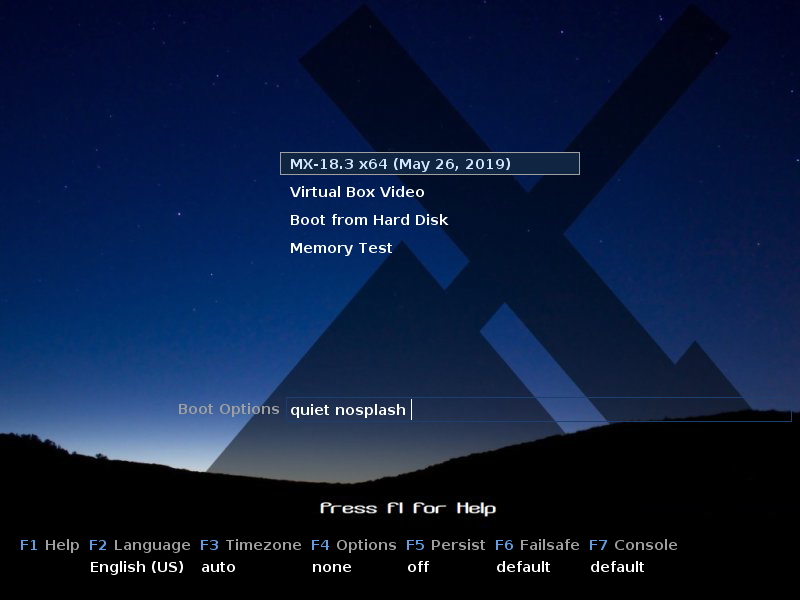
\includegraphics[width=.98\linewidth]{asen/boot}
             \captionof{figure}{Käynnistysvalikko}
              \label{fig:boot}
               \end{minipage}%
               \begin{minipage}{.5\textwidth}
                    \centering
                     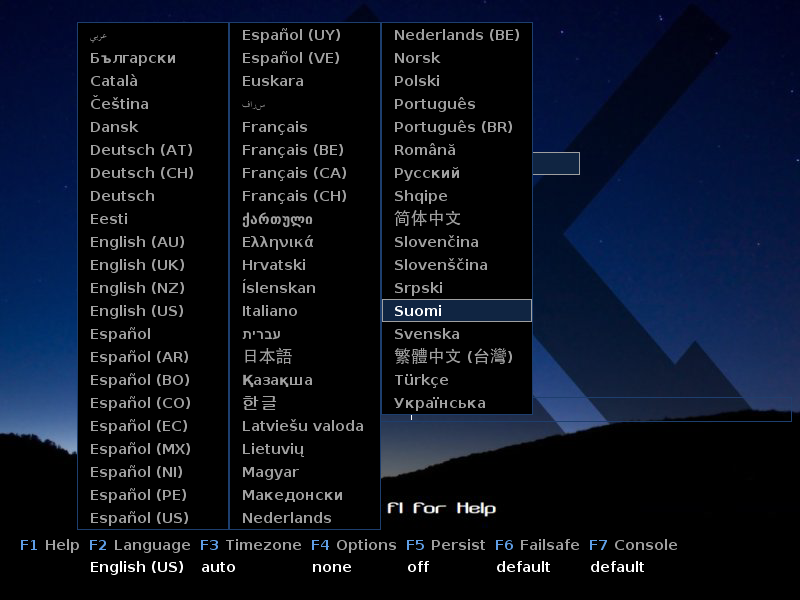
\includegraphics[width=.98\linewidth]{asen/lang}
                      \captionof{figure}{Käynnistysvalikon kieliasetukset}
                       \label{fig:lang}
                        \end{minipage}
                         \end{figure}


Kielen valitsemisen jälkeen jakelun voi käynnistää niin kutsuttuun livetilaan, painamalla Enter-painiketta.

\subsection{Tietoa livetilasta}

Toisin kuin yleisimmät kaupalliset käyttöjärjestelmät, GNU/Linux-jakelut käynnistyvät usein nk. livetilaan, josta jakelu asennetaan.
Livetilassa voi tarkastella järjestelmän ja kovalevyjen tietoja. Mikään tallennettu tiedosto ei kuitenkaan säily käynnistysten välissä. Livetilaa voi hyödyntää esimerkiksi yksityisyyden korostamiseen, tietokoneen korjaamiseen tai jakeluun tutustumiseen ilman varsinaista asennusta. Jakelun käynnistyttyä livetilaan ruudulle ilmestyy Tervetulo-ohjelma.
Tervetulo-ohjelmasta löytyy paljon hyödyllistä tietoa jakelusta ja sen käytöstä. (Kuva \ref{fig:welcome})

\begin{figure}[htpb]
    \begin{center}
        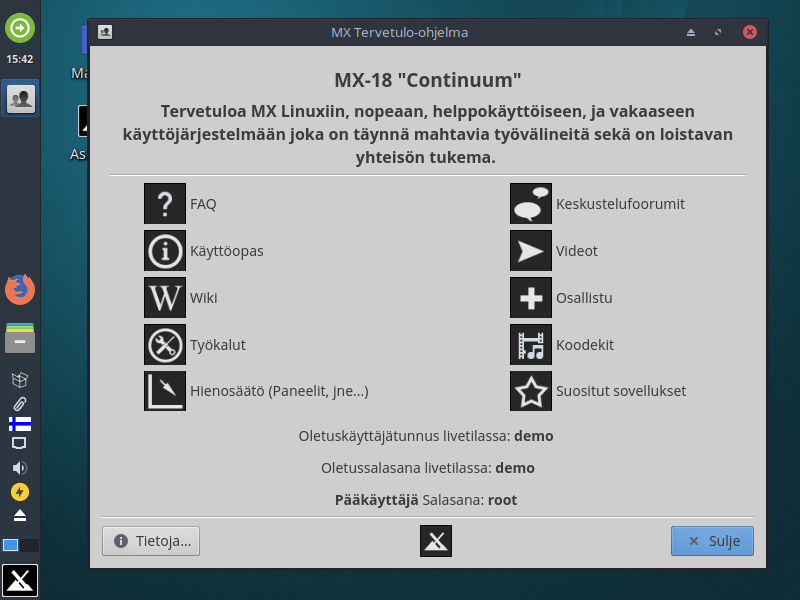
\includegraphics[width=0.9\textwidth]{asen/welcome}
        \caption{Tervetulo-ohjelma}
        \label{fig:welcome}
    \end{center}
\end{figure}

\section{MX Linux 18 -jakelun asentaminen}

Aloittaaksesi asennuksen, sulje kaikki muut sovellukset ikkunoiden oikeasta yläkulmasta. Paikanna asennusohjelma työpöydältä ja avaa se tuplaklikkaamalla sitä kursorilla. (Kuva \ref{fig:asenna})

\begin{figure}[htpb]
    \begin{center}
        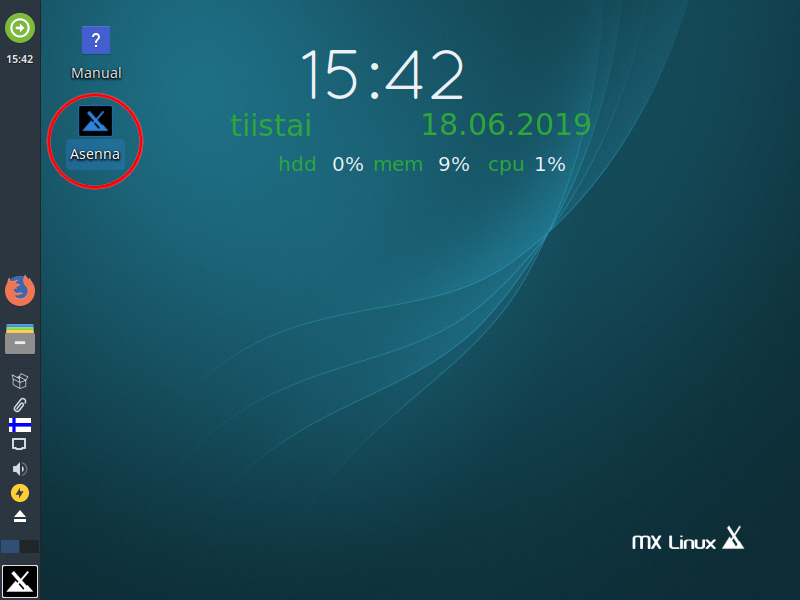
\includegraphics[width=0.875\textwidth]{asen/asenna}
        \caption{Asennusohjelman pikakuvake ympyröitynä}
        \label{fig:asenna}
    \end{center}
\end{figure}

\subsection{Asennusohjelma}

Asennusohjelma käynnistyy perinteisenä ikkunana. Tässä ikkunassa tehdään kaikki tarvittavat määritykset ja lopuksi jakelu asennetaan jakelu kovalevylle.

Ensimmäisessä vaiheessa on lyhyt esittelyteksti sekä näppäimistöasetusten valinta. Mikäli näppäimistön asettelun kohdalla ei lue \textbf{fi}, muuta asettelua painamalla \textit{Muuta näppäimistön asetuksia}. Kun näppäimistön asettelu on vaihdettu sopivaksi, asennusta voi jatkaa painamalla Seuraava-painiketta. (Kuva \ref{fig:as1})

\begin{figure}[htpb]
    \begin{center}
        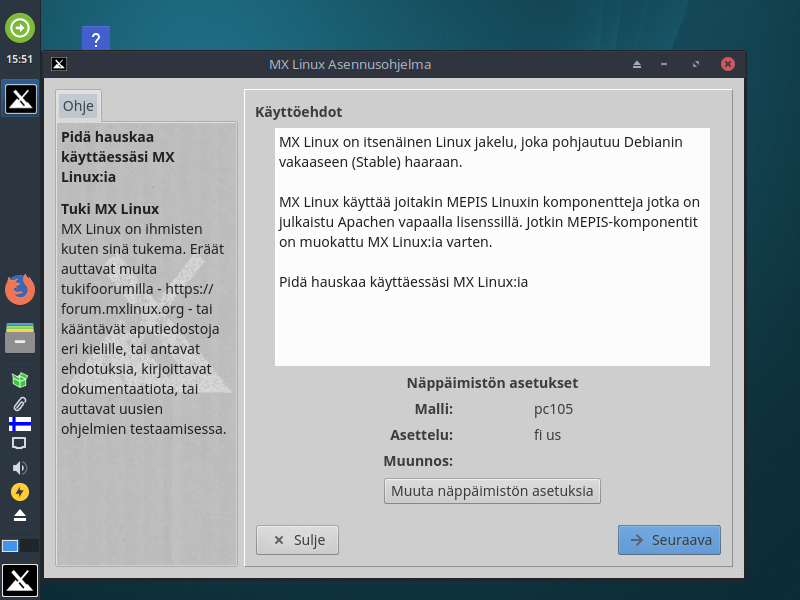
\includegraphics[width=0.875\textwidth]{asen/asennusohjelma1}
        \caption{Asennusohjelman ensimmäinen vaihe}
        \label{fig:as1}
    \end{center}
\end{figure}
\clearpage

\subsection{Osiointi}
Asennusohjelman seuraavassa vaiheessa kovalevy osioidaan. Uusille käyttäjille suositellaan valitsemaan automaattinen osointi valitsemalla kuvassa näkyvän vaihtoehdon \textit{Asenna automaattisesti käyttäen koko levyä}. Tällöin asennusohjelma osioi valitun kovalevyn automaattisesti ja käyttäjän ei tarvitse huolehtia asiasta.
Mikäli olet ennen osioinut GNU/Linux-järjestelmiä ja haluat tehdä sen manuaalisesti, valitse vaihtoehto \textit{Mukautettu asennus olemassaoleville osioille} ja siirry oppaan kohtaan \ref{sec:manual}. (Kuvat \ref{fig:osiointi} ja \ref{fig:auto})

\begin{figure}[htpb]
    \begin{center}
        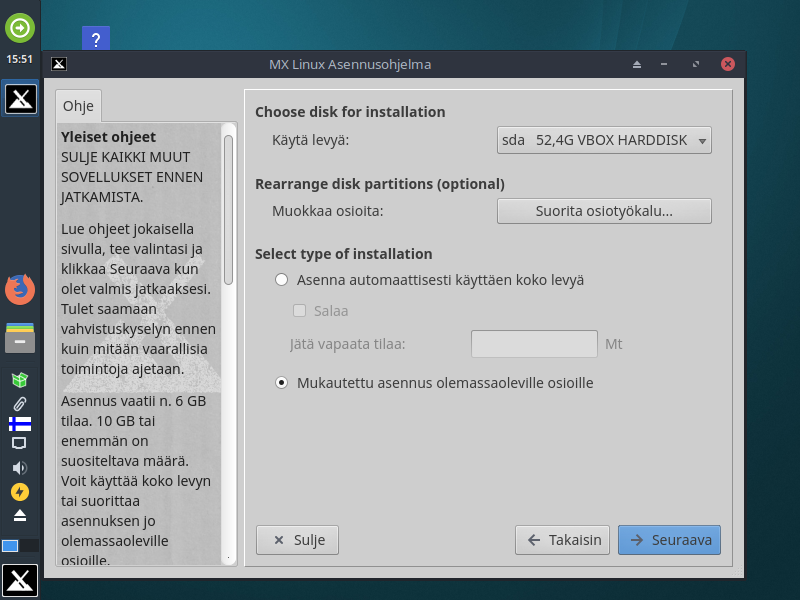
\includegraphics[width=0.7\textwidth]{asen/osiointi}
        \caption{Asennusohjelman osiointivaihe}
        \label{fig:osiointi}
    \end{center}
\end{figure}
\begin{figure}[htpb]
    \begin{center}
        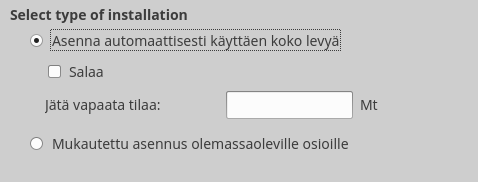
\includegraphics[width=0.65\textwidth]{asen/osiointi_auto}
        \caption{Osiointitavan valitseminen asennusohjelmassa}
        \label{fig:auto}
    \end{center}
\end{figure}


\subsubsection{Manuaalinen osiointi}
\label{sec:manual}
Manuaalista osiointia varten avaa haluamasi osiointityökalu tai suorita \textit{gparted}-työkalu painamalla \textit{Suorita osiotyökalu} -painiketta. Työkalun avauduttua, valitse yläreunasta oikea kovalevy ja poista mahdolliset aikaisemmat osiot painamalla osiota hiiren oikealla painikkeella, ja valitsemalla \textit{poista}. Kuvassa näkyy kovalevy, josta on poistettu jokainen osio, ja on täten valmis osioitavaksi MX Linux 18 -asennusta varten. (Kuva \ref{fig:varaamaton})
\clearpage
\begin{figure}[htpb]
    \begin{center}
        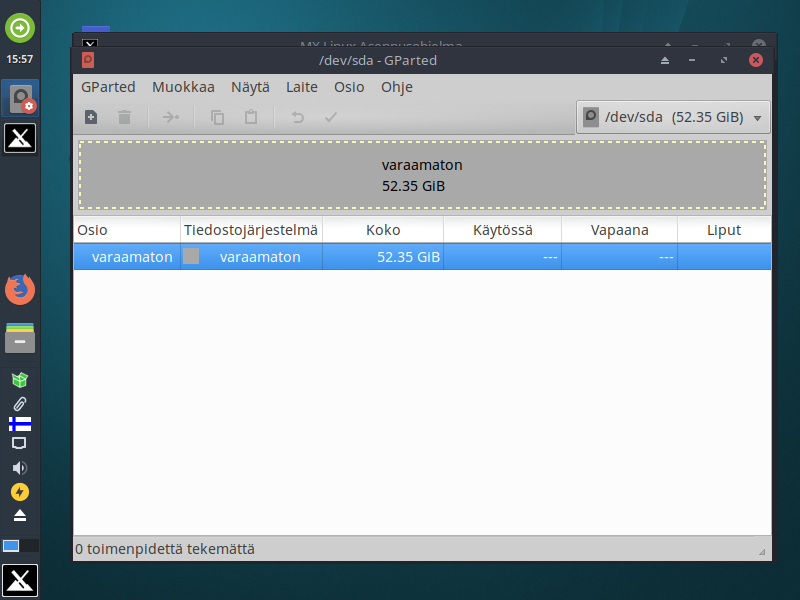
\includegraphics[width=0.98\textwidth]{asen/osiointi_gparted}
        \caption{Gparted-työkalu}
        \label{fig:varaamaton}
    \end{center}
\end{figure}
\begin{wrapfigure}{r}{0.5\textwidth}
  \begin{center}
    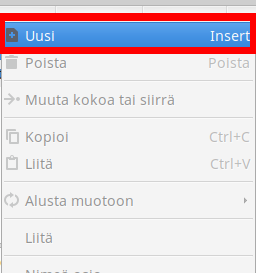
\includegraphics[width=0.35\textwidth]{asen/osiointi_gparted_uusi}
  \end{center}
  \vspace*{-3mm}
  \caption{Uuden osion luominen Gparted\\-työkalun valikosta}
  \label{fig:uusi}
\end{wrapfigure}
Aloita osiointi luomalla swap-osio. Swap tarkoitaa keskusmuistissa olevan tiedon siirtämistä massamuistille, keskusmuistitilan loppuessa.
Swap-osio tehdään mahdollisesti siirrettävää dataa varten. MX Linux 18 suosittelee swap-osion kooksi hieman laitteiston keskusmuistia isompaa määrää. Luo osio painamalla varaamatonta aluetta hiiren oikealla painikkeella ja valitsemalla \textit{uusi}. (Kuva \ref{fig:uusi})
Valitse osion tiedostojärjestelmäksi \textit{linux-swap}.
Aseta myös osion koko. Koko syötetään kohtaan \textit{Uusi koko (MiB)}. Jos laitteessasi on esimerkiksi 8 gigatavua keskusmuistia, anna osion kooksi 8000 MiB. Tässä oppaassa jakelu asennetaan laitteistolla, jossa on kaksi gigatavua keskusmuistia, joten swap-osion koko on 2000 mebitavua eli noin 2,1 gigatavua. (Kuva \ref{fig:swap})
\clearpage
\begin{figure}[htpb]
    \begin{center}
        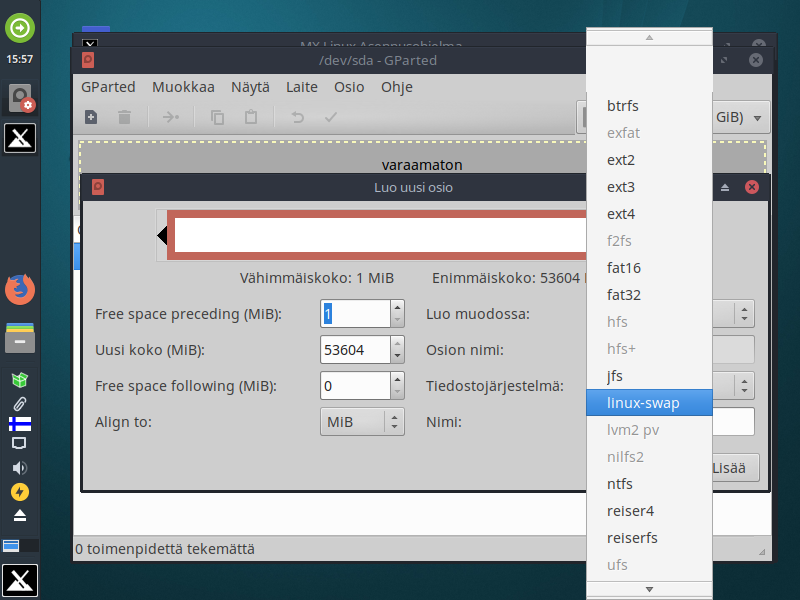
\includegraphics[width=0.7\textwidth]{asen/osiointi_gparted_swap}
        \caption{Swap-osion tiedostojärjestelmä ja koko}
        \label{fig:swap}
    \end{center}
\end{figure}


Luo seuraavaksi juuri-osio. Juuri- eli root-osioon asennetaan varsinainen käyttöjärjestelmä. Osio sisältää kaikki käyttäjän asentamat ohjelmistot ja asetukset. Valitse Gparted-työkalussa varaamaton alue ja paina \textit{Uusi}. Osiolle suositeltu tiedostojärjestelmä on ext4. Osion kooksi suositellaan koko loppu levytilaa. (Kuva \ref{fig:root})

\begin{figure}[htpb]
    \begin{center}
        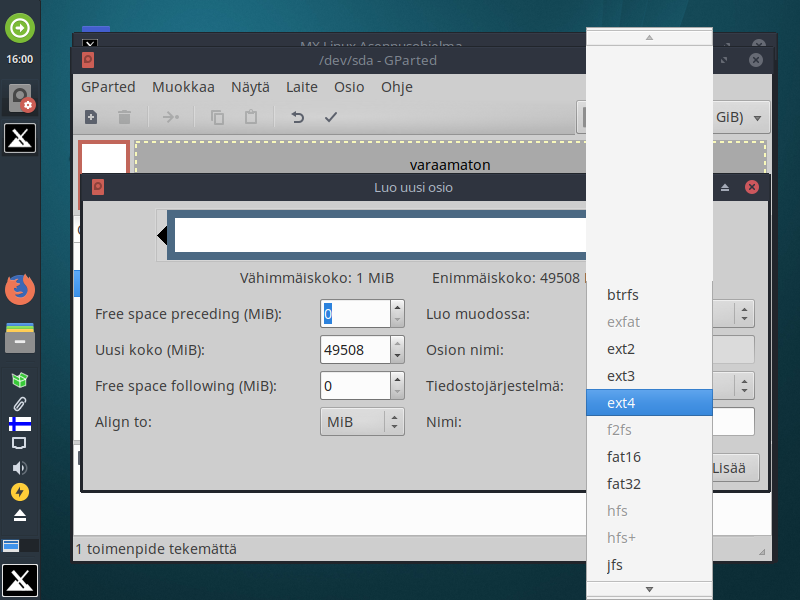
\includegraphics[width=0.7\textwidth]{asen/osiointi_gparted_root}
        \caption{Juuri-osion tiedostojärjestelmä ja koko}
        \label{fig:root}
    \end{center}
\end{figure}

Seuraavaksi tulee liittää luodut osiot oikein. Sulje Gparted-työkalu ja paina asennusohjelmasta Seuraava-painiketta.
Valitse juurerksi luomasi suurempi osio ja varmista, että tyyppi on ext4. Valitse sen jälkeen heittovaihdoksi luomasi swap-osio.
Manuaalinen osiointi on nyt valmis. Jatka asennusta painamalla Seuraava-painiketta. (Kuva \ref{fig:valmis})

\begin{figure}[htpb]
    \begin{center}
        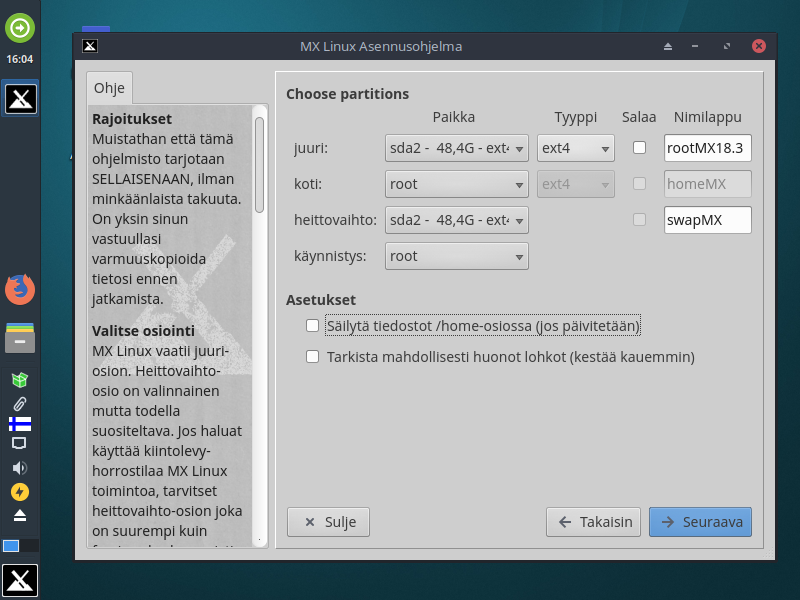
\includegraphics[width=0.98\textwidth]{asen/osiointi_valmis}
        \caption{Osioiden liittäminen asennusohjelmassa}
        \label{fig:valmis}
    \end{center}
\end{figure}

\subsection{GRUB-lataimen asennus}

Seuraavassa vaiheessa asennusohjelma asentaa GRUB-käynnistyslataimen, jota käyttöjärjestelmä käyttää käyttöjärjestelmän käynnistykseen eli lataamiseen. Valitse järjestelmän käynnistyslevyksi sama levy, jolle asennat käyttöjärjestelmän. Mikäli laitteellasi on asennettuna myös Windows-käyttöjärjestelmä, valitse \textit{Asenna GRUB Linuxille ja Windowsille}. Valitse sijainniksi MBR. (Kuva \ref{fig:grub})

\begin{figure}[htpb]
    \begin{center}
        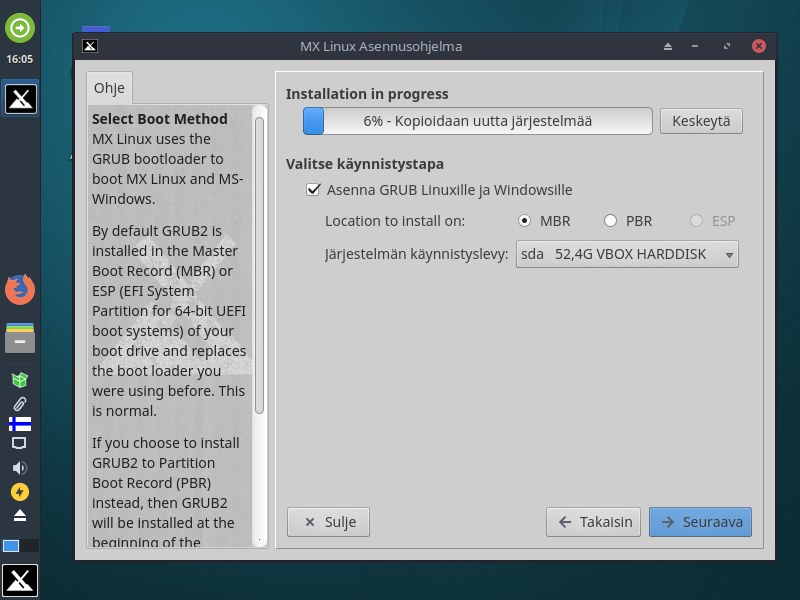
\includegraphics[width=0.98\textwidth]{asen/asennus_grub}
        \caption{GRUB-lataimen asennusvalikko}
        \label{fig:grub}
    \end{center}
\end{figure}
\clearpage
\subsection{Yksilöintiasetukset}

Asennusohjelmassa määritetään laitteelle nimi, verkkonimi ja työryhmä. Nimeä käytetetään yksilöimään tietokone paikallisesti sekä verkossa. Työryhmää käytetään työskentelyyn vertaisverkossa. Mikäli et tiedä mitä sinun tulisi syöttää näihin, jätä ne muuttamatta. (Kuva \ref{fig:hosts})

\begin{figure}[htpb]
    \begin{center}
        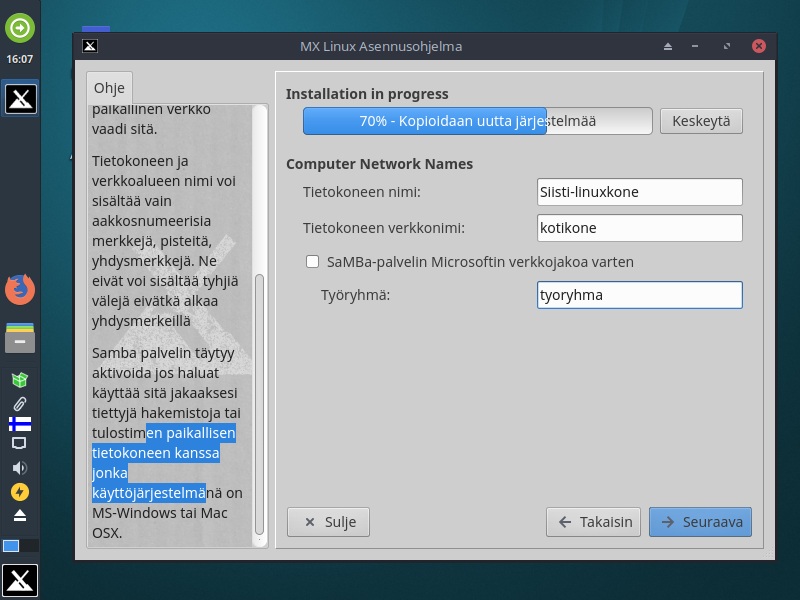
\includegraphics[width=0.98\textwidth]{asen/asennus_hosts}
        \caption{Tietokoneen eri yksilöintiasetusten määritys asennusohjelmassa}
        \label{fig:hosts}
    \end{center}
\end{figure}
\clearpage
\subsection{Sijainti- ja kelloasetukset}

Asennusohjelma kysyy käyttäjän sijaintia ja aikavyöhykettä. Syötä haluamasi sijainti ja aikavyöhyke. Voit myös valita, haluatko käyttää 12 vai 24 tunnin kelloa. Kuvassa näkyy esimerkkiasetukset. (Kuva \ref{fig:locale})

\begin{figure}[htpb]
    \begin{center}
        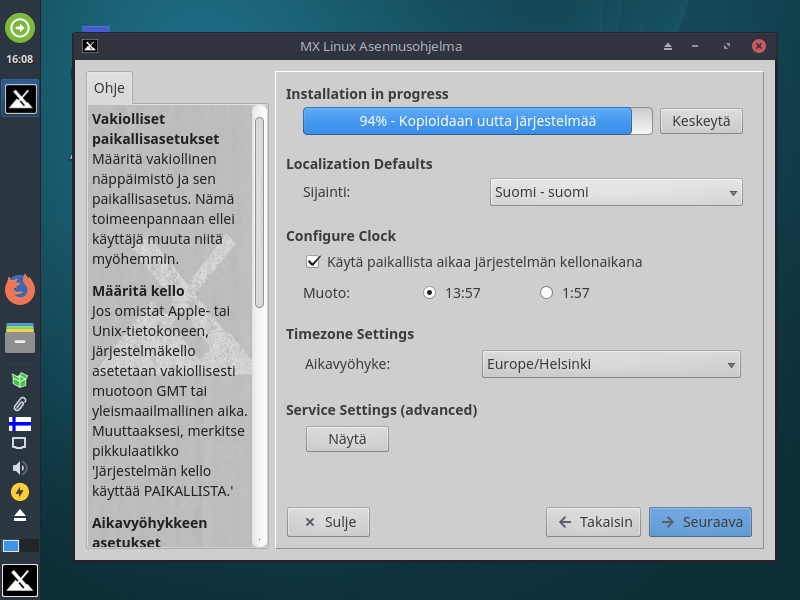
\includegraphics[width=0.98\textwidth]{asen/asennus_locale}
        \caption{Esimerkkiasetukset sijaintiasetuksiin asennusohjelmassa}
        \label{fig:locale}
    \end{center}
\end{figure}

\subsection{Käyttäjätilin luonti}

Viimeiseksi asennusohjelmassa luodaan käyttäjätili ja annetaan pääkäyttäjälle salasana. Luo oma käyttäjätilisi haluamallasi käyttäjänimellä ja salasanalla.
Pääkäyttäjän salasanan tulisi olla turvallinen ja vain laitteen hallitsijan tiedossa.
Pääkäyttäjäsalasanaa tarvitaan muun muassa silloin, kun halutaan asentaa tai päivittää ohjelmia, päivittää käyttöjärjestelmä tai sen osia tai poistaa suojattuja ohjelmia ja tiedostoja. (Kuva \ref{fig:user})
\\

Asennus on nyt valmis. Käynnistä laitteesi uudelleen valitsemalla automaattinen uudelleenkäynnistys ja painamalla asennusohjelman \textit{Lopeta}-painiketta. (Kuva \ref{fig:valmis2})

\begin{figure}[htpb]
    \begin{center}
        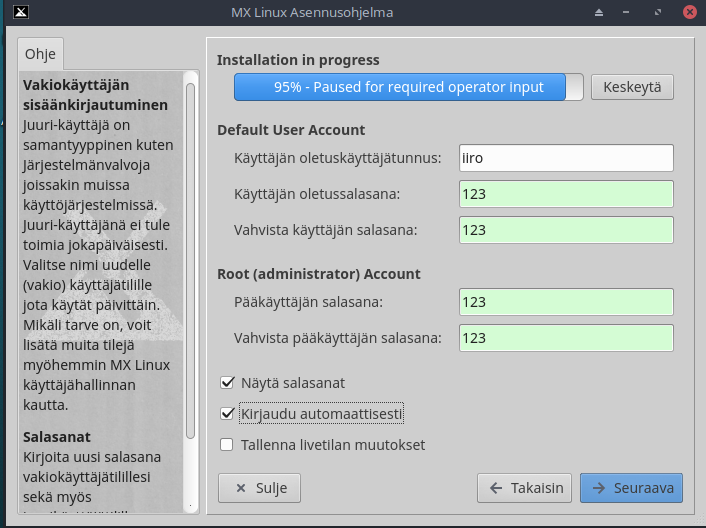
\includegraphics[width=0.899\textwidth]{asen/asennus_user}
        \caption{Käyttäjätilin luonti asennusohjelmassa}
        \label{fig:user}
    \end{center}
\end{figure}

\begin{figure}[htpb]
    \begin{center}
        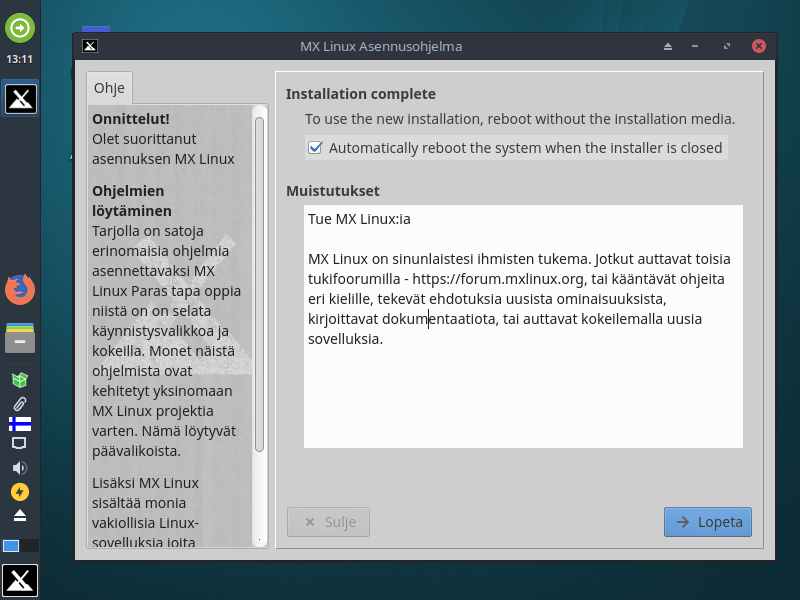
\includegraphics[width=0.899\textwidth]{asen/asennus_valmis}
        \caption{Asennusohjelma valmistuneena}
        \label{fig:valmis2}
    \end{center}
\end{figure}

\section{Peruskäyttö}

\subsection{Työpöytäympäristö}
MX Linuxin työpöytää hallitaan vasemmalla sijaitsevasta palkista, josta löytyy muun muassa sovellusvalikko, uloskirjautumis- ja sammutus-painike, avoimet ikkunat ja pikakuvakkeita sovelluksiin.
(Kuva \ref{fig:tyopoytaymparisto})

\begin{figure}[htpb]
    \begin{center}
        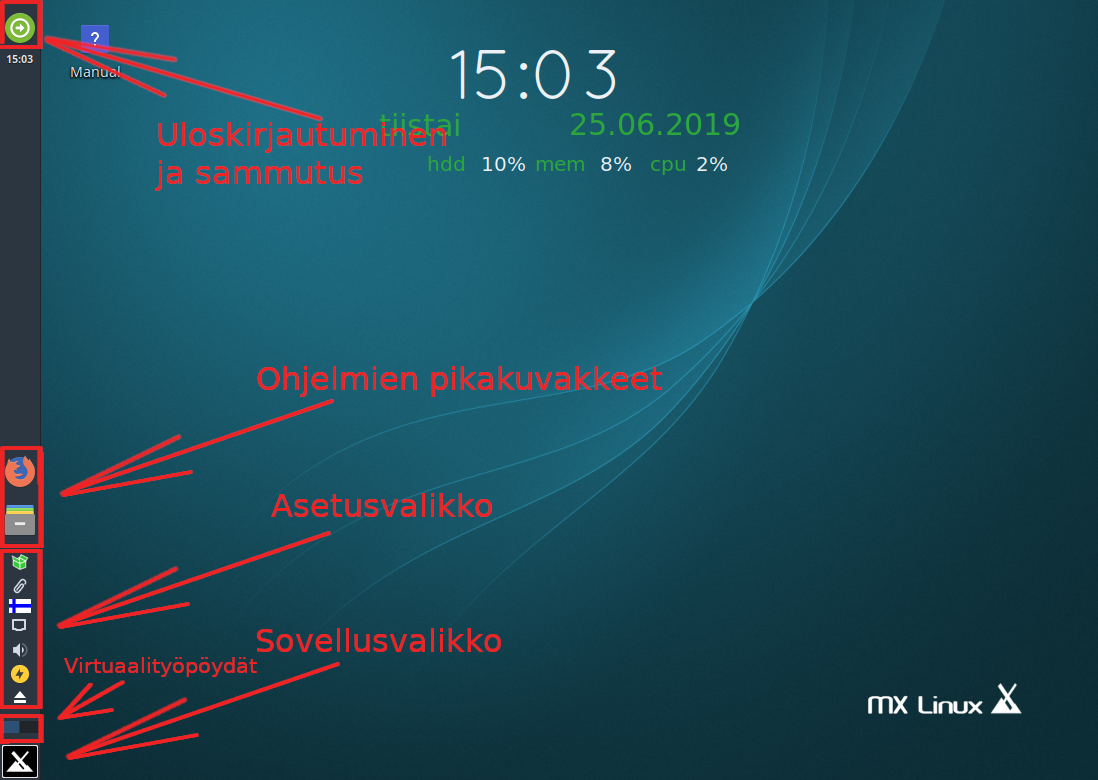
\includegraphics[width=0.98\textwidth]{ymparisto/tyopoyta}
        \caption{Työpöytäympäristö ja sivupalkin selitykset}
        \label{fig:tyopoytaymparisto}
    \end{center}
\end{figure}
\clearpage

\subsection{Internet}

Mikäli käytät langallista verkkoyhteyttä, MX Linuxin tulisi yhdistää verkkoon automaattisesti. Jos näin ei tapahdu avaa verkkoasetukset avaamalla sovellusvalikko (Kuva \ref{fig:valikko}) ja hakemalla \textit{verkkoyhteydet}. (Kuva \ref{fig:verkko})
\begin{figure}[htbp]
     \centering
      \begin{minipage}{.60\textwidth}
           \centering
            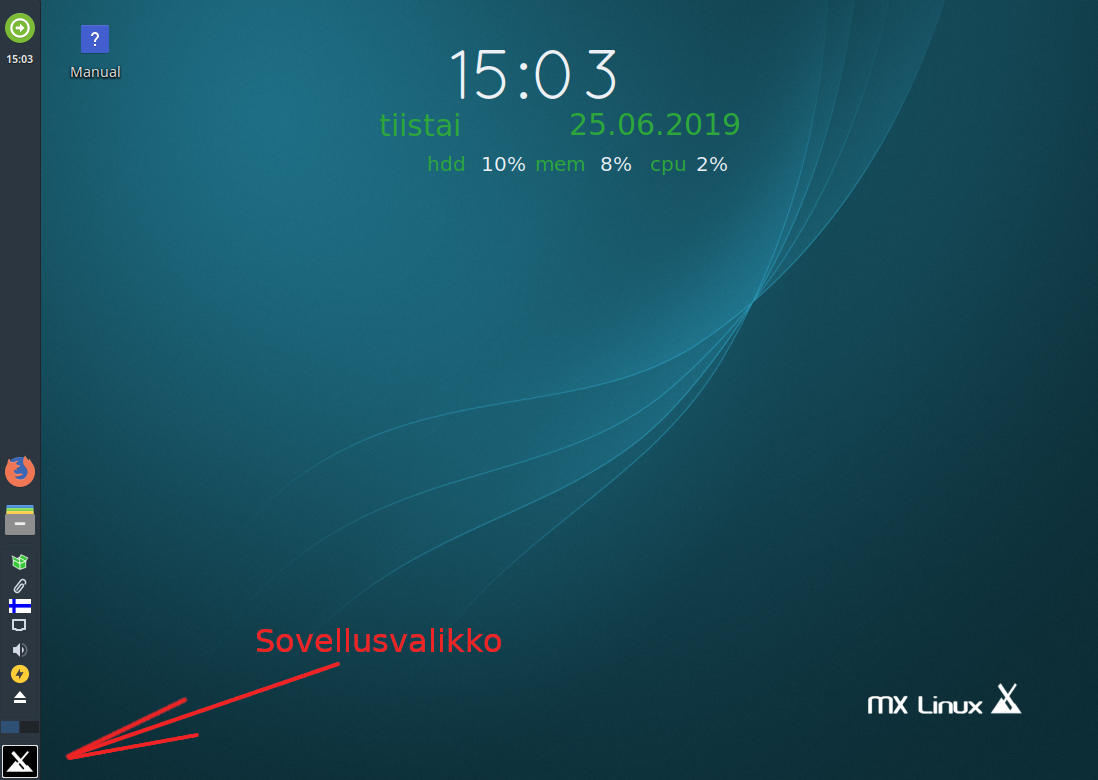
\includegraphics[width=.98\linewidth]{internet/tyopoyta}
             \captionof{figure}{Sovellusvalikon painike sivupalkissa}
              \label{fig:valikko}
               \end{minipage}%
               \begin{minipage}{.40\textwidth}
                    \centering
                     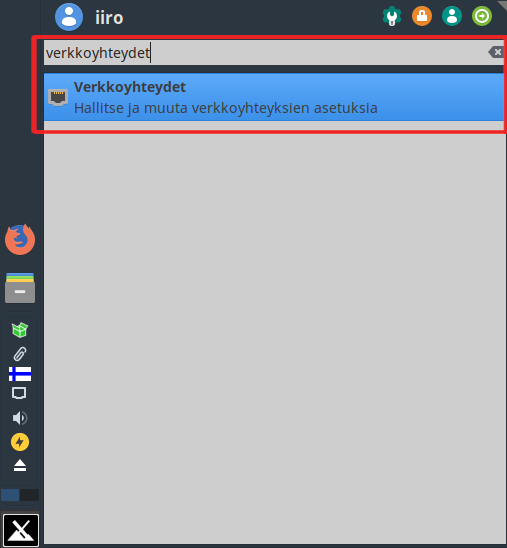
\includegraphics[width=.98\linewidth]{internet/verkkoyhteydet}
                      \captionof{figure}{MX Linuxin sovellusvalikossa hakeminen}
                       \label{fig:verkko}
                        \end{minipage}
                         \end{figure}


Verkkoyhteys asetukset avautuu. Paina \textit{Lisää}-painiketta, lisätäksesi uuden yhteyden. (Kuva \ref{fig:vasetukset}) Langallista yhteyttä varten valitse yhteyden tyypiksi \textit{Ethernet}. (Kuva \ref{fig:ethernet})
Tallenna yhteys vakioasetuksilla ja laitteesi on yhdistetty verkkoon (Kuva \ref{fig:connection})

\begin{figure}[htbp]
     \centering
      \begin{minipage}{.5\textwidth}
           \centering
            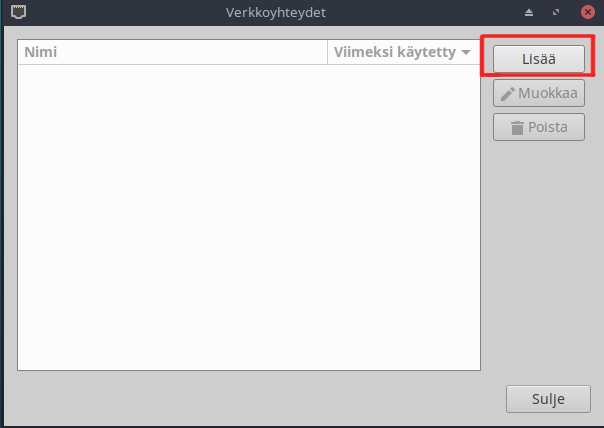
\includegraphics[width=.98\linewidth]{internet/lisaa_yhteys}
             \captionof{figure}{Sovellusvalikon painike sivupalkissa}
              \label{fig:vasetukset}
               \end{minipage}%
               \begin{minipage}{.5\textwidth}
                    \centering
                     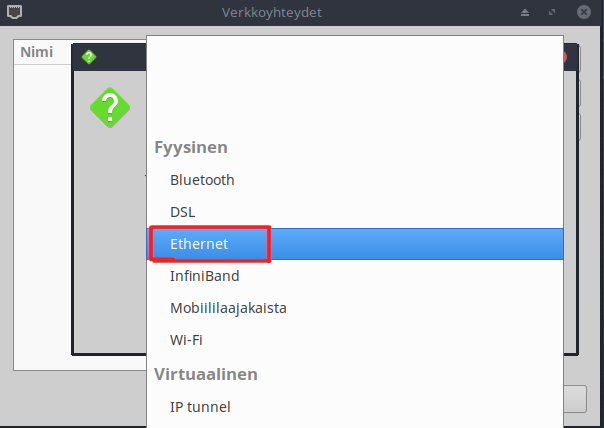
\includegraphics[width=.98\linewidth]{internet/yhteys_ethernet}
                      \captionof{figure}{MX Linuxin sovellusvalikossa hakeminen}
                       \label{fig:ethernet}
                        \end{minipage}
                         \end{figure}
                         \clearpage


\begin{figure}[htpb]
    \begin{center}
        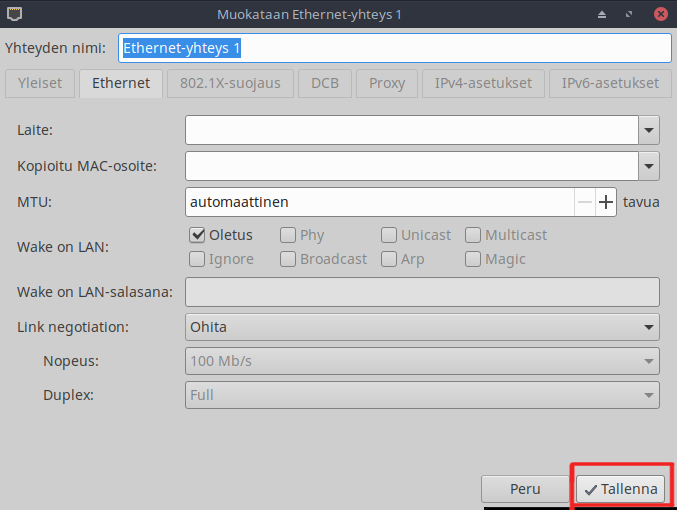
\includegraphics[width=0.8\textwidth]{internet/yhteys_tallenna}
        \caption{Verkkoyhteyden tallentaminen}
        \label{fig:connection}
    \end{center}
\end{figure}

\subsubsection{Selain}
\begin{wrapfigure}{r}{0.5\textwidth}
  \begin{center}
    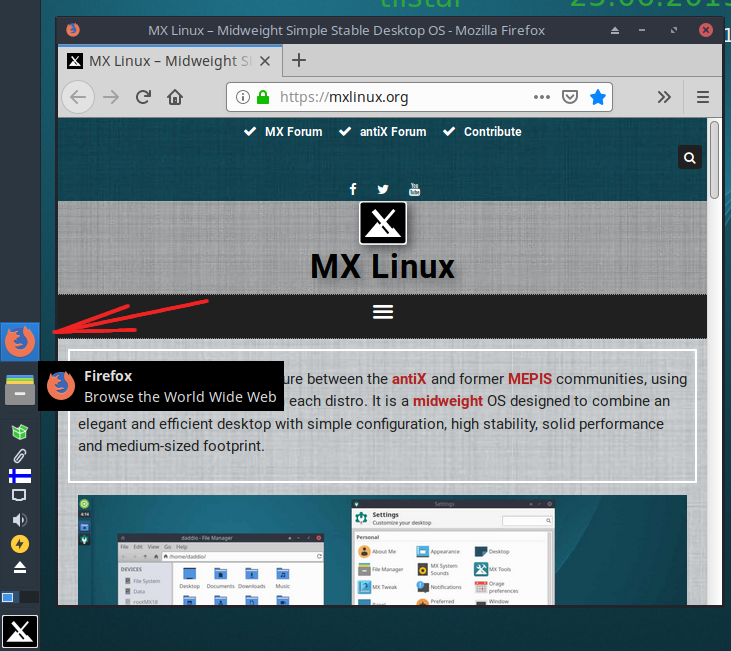
\includegraphics[width=0.5\textwidth]{internet/firefox}
  \end{center}
  \vspace*{-3mm}
  \caption{Mozilla Firefox -selain ja sen pikakuvake}
  \label{fig:firefox}
\end{wrapfigure}

MX Linuxissa on valmiiksi asennettuna \textit{Mozilla Firefox} -selain. Jos haluat käyttää jotain muuta selainta, sovelluskaupasta löytyy paljon selainvaihtoehtoja, joita voi asentaa ilmaiseksi.
Löydät valmiiksi asennetun selaimen pikakuvakkeen sivupalkista. (Kuva \ref{fig:firefox})

\subsection{Ohjelmien hallinta}
Sillä MX Linux pohjautuu suosituimpaan GNU/Linux-jakeluun, sille on tarjolla valtavasti ohjelmia. Ohjelmia voi hakea Internetistä tai MX Linuxin paketinhallintaohjelmasta.
Suositeltu tapa asentaa ja hallita ohjelmia MX Linuxilla on joko asentaa ne terminaalista tai käyttää ns. paketinhallintaohjelmaa.
Paketinhallintaohjelmat toimivat teoriassa samalla tavalla, kuin paketinhallintatyökalun käyttö terminaalissa. MX Linux käyttää apt-paketinhallintajärjestelmää. Järjestelmään on asennettu valmiiksi Synaptic-niminen paketinhallintaohjelma, jossa on graafinen käyttöliittymä.

\clearpage
\subsubsection{Synaptic-paketinhallintaohjelma}
Löydät Synaptic-ohjelman hakemalla sovellusvalikosta hakusanalla \textit{synaptic}.
(Kuva \ref{fig:synaptichaku})
Huomioi, että ohjelma vaatii käynnistyäkseen pääkäyttäjän salasanan.

\begin{figure}[htpb]
    \begin{center}
        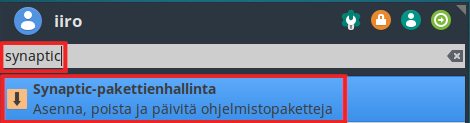
\includegraphics[width=0.65\textwidth]{ymparisto/synaptic_haku}
        \caption{Synaptic-ohjelma sovellusvalikossa}
        \label{fig:synaptichaku}
    \end{center}
\end{figure}

Synaptic-ohjelmassa voit asentaa, päivittää ja poistaa paketteja, eli ns. ohjelmia. Ohjelman avauduttua, näet näkymän, jossa voit etsiä eri paketteja sekä poistaa, asentaa, päivittää ja selata niitä. (Kuva \ref{fig:syn_nak})

\begin{figure}[htpb]
    \begin{center}
        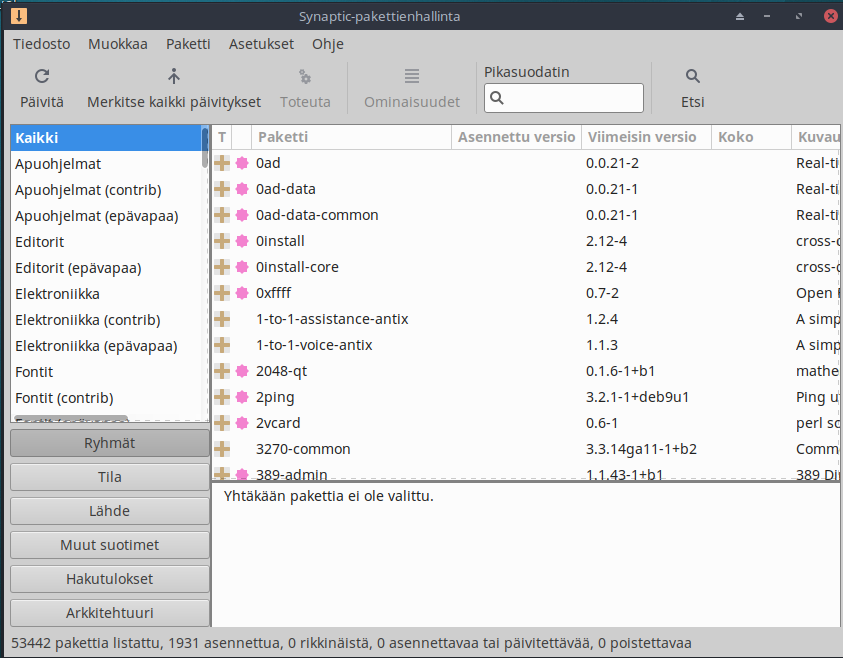
\includegraphics[width=0.7\textwidth]{ymparisto/synaptic_nakyma}
        \caption{Synaptic-ohjelman perusnäkymä}
        \label{fig:syn_nak}
    \end{center}
\end{figure}

Esimerkiksi Chromium-selaimen asentaminen tapahtuisi hakemalla \textit{Etsi}-painikkeella "\textit{chromium}". (Kuva \ref{fig:chro_haku})
Tämän jälkeen paikannetaan oikea paketti hakutuloksista. Tässä tapauksessa oikea paketti on nimeltään \textit{chromium}. Vie kursori paketin nimen päälle ja avaa lisävalikko painamallla hiiren oikeaa painiketta, ja valitse \textit{Merkitse asennettavaksi}. (Kuva \ref{fig:chro_menu})

\begin{figure}[htpb]
    \begin{center}
        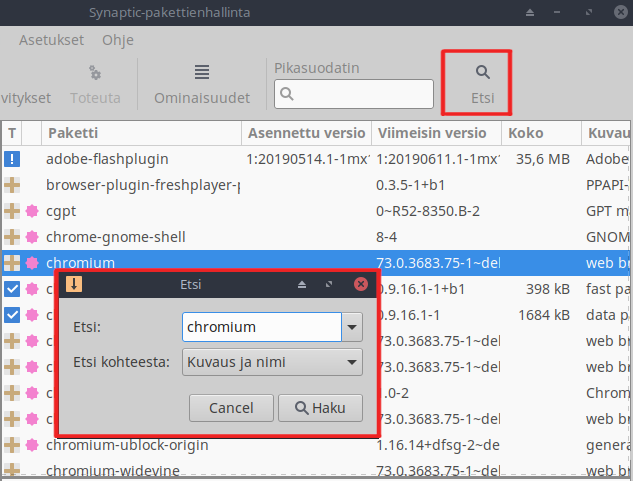
\includegraphics[width=0.85\textwidth]{ymparisto/chro_haku}
        \caption{Paketin hakeminen Synaptic-ohjelmassa}
        \label{fig:chro_haku}
    \end{center}
\end{figure}

\begin{figure}[htpb]
    \begin{center}
        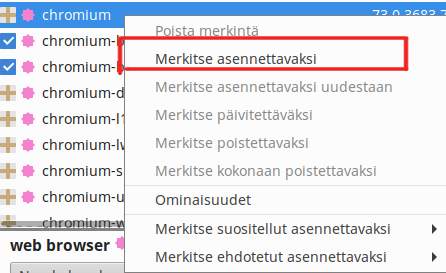
\includegraphics[width=0.85\textwidth]{ymparisto/chro_menu}
        \caption{Paketin lisävalikko}
        \label{fig:chro_menu}
    \end{center}
\end{figure}
\clearpage

Paina tämän jälkeen \textit{Toteuta}-painiketta ylävalikosta. (Kuva \ref{fig:toteuta}) Huomoi, että voit merkitä niin monta pakettia asennettavaksi, kuin haluat. Säästät näin aikaa, asentaessasi isompia määriä paketteja kerralla.

\begin{figure}[htpb]
    \begin{center}
        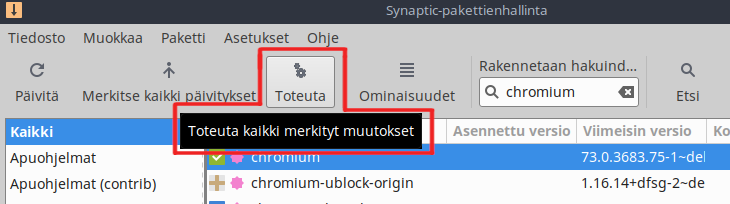
\includegraphics[width=0.756\textwidth]{ymparisto/syn_toteuta}
        \caption{Asennuksen toteutuspainike Synaptic-ohjelman ylävalikossa}
        \label{fig:toteuta}
    \end{center}
\end{figure}

Ohjelma kysyy käyttäjän varmistusta. Viimeistelläksesi asentamisen, paina \textit{Apply}-painiketta alakulmasta. (Kuva \ref{fig:toteuta2}) Chromium-selain löytyy nyt sovellusvalikostasi.

\begin{figure}[htpb]
    \begin{center}
        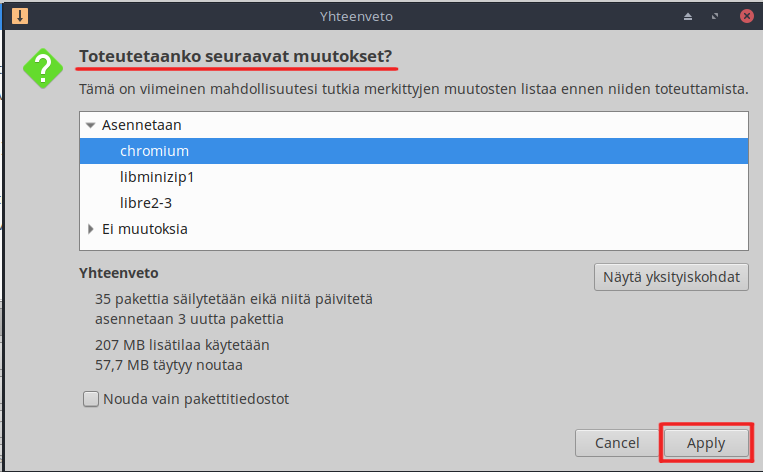
\includegraphics[width=0.756\textwidth]{ymparisto/syn_toteuta2}
        \caption{Asennuksen varmistaminen}
        \label{fig:toteuta2}
    \end{center}
\end{figure}

\clearpage

\subsubsection{Apt-paketinhallinta terminaalista}
Ohjelmien ja työkalujen käyttäminen terminaalista on tehokasta, mutta yleensä suositeltavaa vain kokeneemmille käyttäjille.

MX Linuxissa on valmiina asetettu pikanäppäin terminaalin avaamiselle. Voit avata terminaliin painamalla F4-näppäintä. Terminaali aukeaa työpöydän yläpuolelta. (Kuva \ref{fig:terminal})
\begin{figure}[htpb]
    \begin{center}
        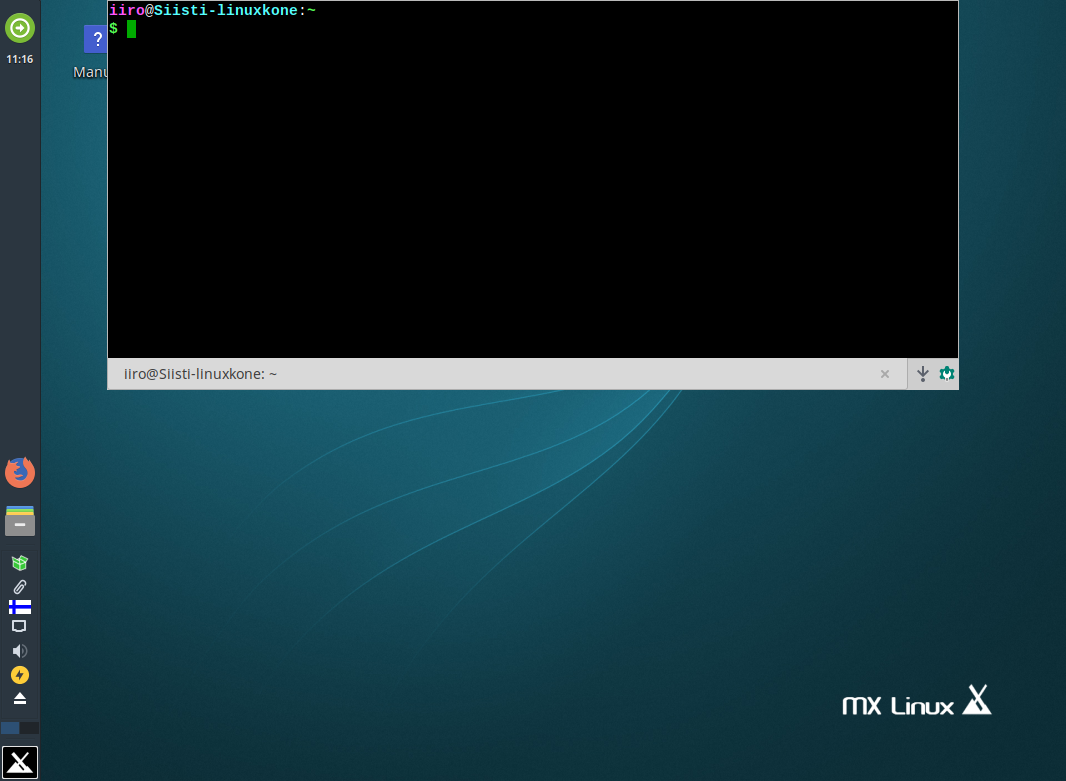
\includegraphics[width=0.866\textwidth]{ymparisto/terminal}
        \caption{Terminaali avattuna}
        \label{fig:terminal}
    \end{center}
\end{figure}

Ohjelman asentaminen tapahtuu seuraavalla komennolla:
\begin{lstlisting}
sudo apt-get install paketinnimi
\end{lstlisting}

Tämä on tehokkain tapa asentaa paketteja, mikäli tiedät niiden nimen jo valmiiksi. Komennon voi jakaa osiin. \textbf{sudo} on komento jolla saadaan toteutettua seuraava komento pääkäyttäjän oikeuksilla. \textbf{Apt-get} on Apt-paketinhallintatyökalun komento, ja sen jälkeen kerrotaan sille, mitä halutaan tehdä. Tässä tapauksessa apt-get-komennon jälkeen kirjoitetaan \textbf{install}, sillä tarkoituksena on asentaa paketti. Muita vaihtoehtoja on mm. \textit{remove}, \textit{purge} ja \textit{update}. Viimeiksesi annetaan paketin nimi.

Esimerkki chromium-paketin asentamisesta terminaalissa:
\begin{lstlisting}
    sudo apt-get install chromium
\end{lstlisting}

\subsection{Järjestelmän päivittäminen}
MX Linuxiin on rakennettu sisään päivitysohjelma, joka ilmoittaa saatavilla olevista päivityksistä ja tarjoaa näiden päivitysten asentamista. Päivitysohjelma on hyvin intiutiivinen ja siihen löytyy erillinen käyttöopas jakelun kotisivuilta. On hyvä kuitenkin itse ymmärtää, kuinka päivittää järjestelmä terminaalista. Kuten pakettien hallitsemiseenkin, siihen käytetään Apt-työkalua. Voit päivittää tietokoneesi esimerkiksi näin:
\begin{lstlisting}
    sudo apt-get update && sudo apt-get upgrade
\end{lstlisting}
Tämä hakee viimeisimmän version jokaisesta asennetusta paketista, työkalusta ja järjestelmän osasta ja sen jälkeen suorittaa \textit{upgrade}-komennon, joka päivittää paketit, joille on tarjolla päivitys. Komento vaatii toimivan Internet-yhteyden sekä pääkäyttäjän oikeudet.

\subsection{Työohjelmat}

MX Linuxille ei ole saatavilla suosituimpia kaupallisia työohjelmia. Hyviä vapaan lähdekoodin vaihtoehtoja kuitenkin löytyy runsaasti. Vapaan lähdekoodin työohjelmat eivät useimmiten sovi ammattimaiseen työskentelyyn, ominaisuuksien ja tuen puutteen vuoksi.
Alla on taulukko, jossa näkyy kaupallinen ohjelma ja sen suosituin ilmainen korvaaja.

\begin{table}[ht]
\caption{Vaihtoehtoja kaupallisille työohjelmille}
\label{tab:oss}
    \begin{center}
\begin{tabular}{ll}
\textbf{Kaupallinen ohjelma}              & \textbf{Ilmainen vaihtoehto} \\ \hline
\multicolumn{1}{l|}{Microsoft Word}       & LibreOffice Writer           \\
\multicolumn{1}{l|}{Microsoft PowerPoint} & LibreOffice Impress          \\
\multicolumn{1}{l|}{Microsoft Excel}      & LibreOffice Calc             \\
\multicolumn{1}{l|}{Adobe Photoshop}      & GIMP
\end{tabular}
    \end{center}
\end{table}

\subsection{Ulkoasun kustomointi}

MX Linuxin kustomointimahdollisuudet ovat verrattain suuret. Voit muuttaa lähes jokaista asiaa työpöytäympäristössäsi. Internet on täynnä ohjeita Linux-järjestelmien kustomointiin. Tässä osiossa käydään läpi yleisimmät ulkoasukustomoinnit.

\subsubsection{Taustakuvan vaihtaminen}

Vaihtaaksesi taustakuvan, avaa asetukset. Voit avata asetukset hakemalla sovellusvalikosta hakusanalla \textit{asetukset}. Valitse asetuksista kohta työpöytä. (Kuva \ref{fig:taustakuva1}) Voit valita taustakuvan useista järjestelmän mukana tulleista taustakuvista. (Kuva \ref{fig:taustakuva2}) Voit myös valita kuvan omasta hakemistostasi, kuten ladatuista kuvista. (Kuva \ref{fig:taustakuva3})

\begin{figure}[htpb]
    \begin{center}
        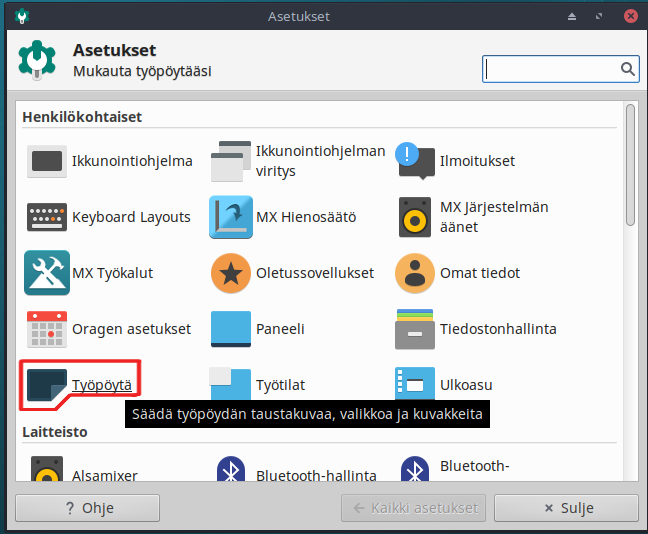
\includegraphics[width=0.75\textwidth]{taustakuva}
        \caption{Asetusvalikko}
        \label{fig:taustakuva1}
    \end{center}
\end{figure}

\begin{figure}[htpb]
    \begin{center}
        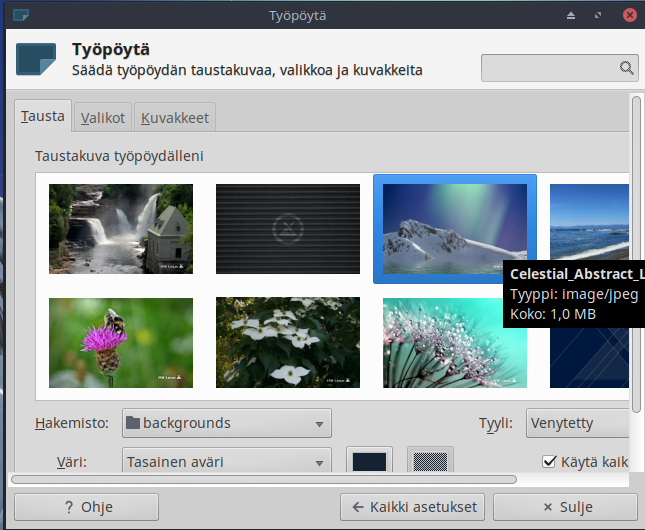
\includegraphics[width=0.75\textwidth]{taustakuva_valittu}
        \caption{Uusi taustakuva valittuna}
        \label{fig:taustakuva2}
    \end{center}
\end{figure}

\begin{figure}[htpb]
    \begin{center}
        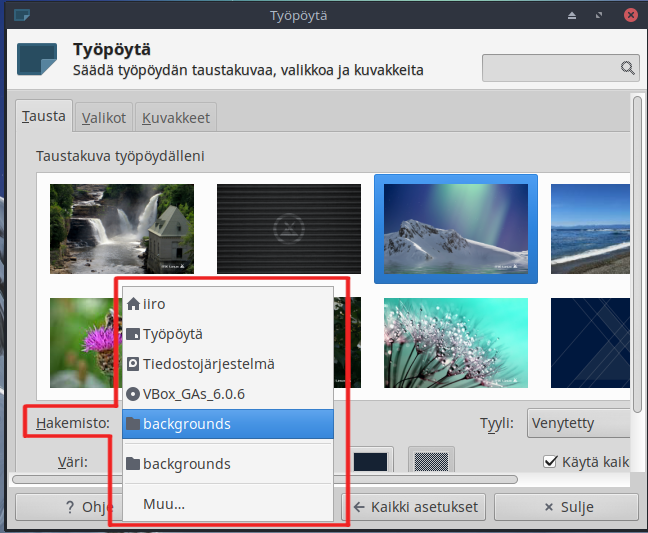
\includegraphics[width=0.75\textwidth]{taustakuva_hakemisto}
        \caption{Hakemiston vaihtaminen taustakuva-asetuksissa}
        \label{fig:taustakuva3}
    \end{center}
\end{figure}
\section{Ylläpito}
\subsection{Käyttäjien hallinta}
Mikäli laitetta käyttää useampi ihminen, useamman käyttäjän sisällyttäminen on suositeltua. Jos laitteellasi on tällä hetkellä vain asennusvaiheessa luotu käyttäjätili, voit luoda uuden avaamalla MX Käyttäjänhallinta -ohjelman. (Kuva \ref{fig:hallinta})

\begin{figure}[htpb]
    \begin{center}
        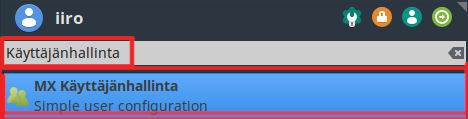
\includegraphics[width=0.5\textwidth]{user/set}
        \caption{MX Käyttäjänhallinta -ohjelma sovellusvalikossa}
        \label{fig:hallinta}
    \end{center}
\end{figure}

Ohjelman avauduttua voit heti luoda uuden käyttäjän syöttämällä tiedot kolmeen ensimmäiseen tekstikenttään, jotka ovat rajattuna kuvassa punaisella. Keltaisella rajatusta kohdasta, voit poistaa olemassaolevia käyttäjiä. (Kuva \ref{fig:usernak})

Mikäli haluat antaa jollekkin käyttäjälle oikeuden käyttää \textit{sudo}-komentoa, eli mahdollisuuden käyttää pääkäyttäjän oikeuksia, siirry välilehteen \textit{Ryhmän jäsenyys}. Valitse sen jälkeen muokattava käyttäjä ja valitse ruksittamalla kohta \textbf{sudo}. (Kuva \ref{fig:group})

Kaikkien tekemiesi muutosten jälkeen paina alareunasta \textit{Hyväksy}-painiketta, tallentaaksesi muutokset.

\begin{figure}[htpb]
    \begin{center}
        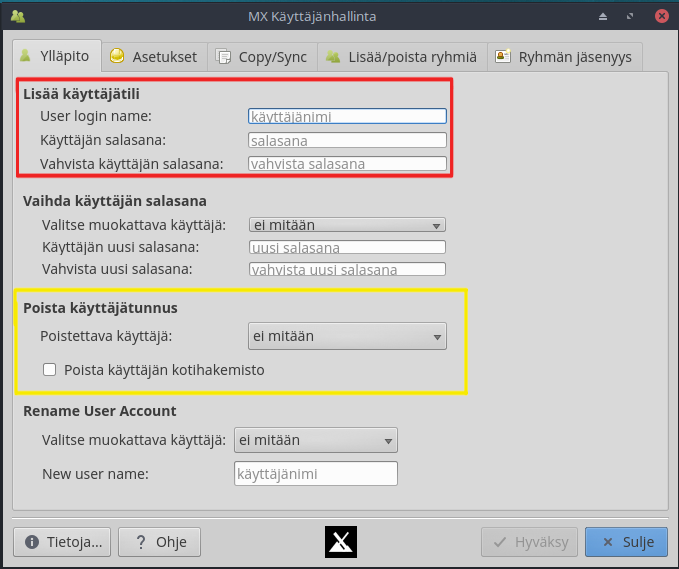
\includegraphics[width=0.8\textwidth]{user/nakyma}
        \caption{MX Käyttäjänhallinta -ohjelman perusnäkymä}
        \label{fig:usernak}
    \end{center}
\end{figure}
\begin{figure}[htpb]
    \begin{center}
        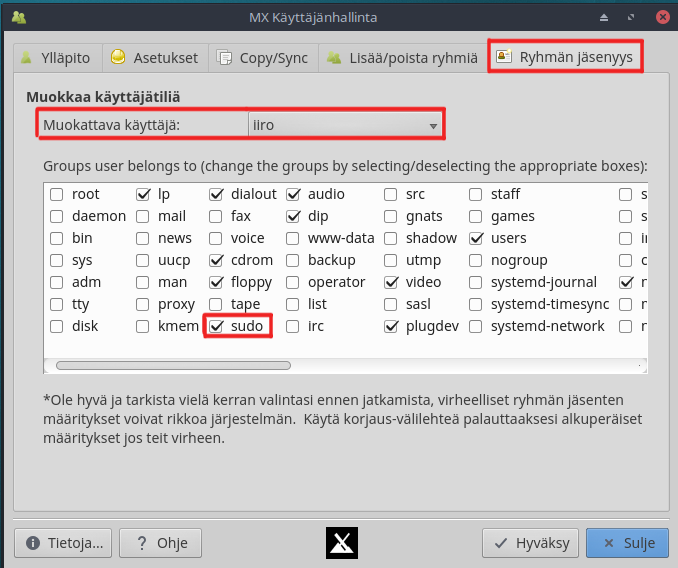
\includegraphics[width=0.8\textwidth]{user/group}
        \caption{Ryhmän jäsenyys -välilehti}
        \label{fig:group}
    \end{center}
\end{figure}


\end{document}

